% options:
% thesis=B bachelor's thesis
% thesis=M master's thesis
% czech thesis in Czech language
% slovak thesis in Slovak language
% english thesis in English language
% hidelinks remove colour boxes around hyperlinks

\documentclass[thesis=M,czech]{FITthesis}[2014/05/07]

\usepackage[utf8]{inputenc} % LaTeX source encoded as UTF-8

\usepackage{graphicx} %graphics files inclusion
% \usepackage{amsmath} %advanced maths
% \usepackage{amssymb} %additional math symbols

\usepackage{dirtree} %directory tree visualisation

\usepackage{nameref}

% % list of acronyms
% \usepackage[acronym,nonumberlist,toc,numberedsection=autolabel]{glossaries}
% \iflanguage{czech}{\renewcommand*{\acronymname}{Seznam pou{\v z}it{\' y}ch zkratek}}{}
% \makeglossaries

\newcommand{\tg}{\mathop{\mathrm{tg}}} %cesky tangens
\newcommand{\cotg}{\mathop{\mathrm{cotg}}} %cesky cotangens

% % % % % % % % % % % % % % % % % % % % % % % % % % % % % % 
% ODTUD DAL VSE ZMENTE
% % % % % % % % % % % % % % % % % % % % % % % % % % % % % % 

\department{Katedra softwarového inženýrství}
\title{Adaptibilní systém pro doporučování obsahu}
\authorGN{Jan} %(křestní) jméno (jména) autora
\authorFN{Bouchner} %příjmení autora
\authorWithDegrees{Bc. Jan Bouchner} %jméno autora včetně současných akademických titulů
\supervisor{Ing. Jaroslav Kuchař}
\acknowledgements{Chci upřímně poděkovat všem, kteří mi věnovali čas, když jsem potřeboval pomoci při psaní této práce, především vedoucímu práce Jaroslavu Kuchaři za správné směrování, celkový vhled do technologií, cenné komentáře a nové nápady, které pomohly ke vzniku této práce. Děkuji také své rodině a přátelům za bezvýhradnou podporu během celých mých studií.}
\abstractCS{V~několika větách shrňte obsah a přínos této práce v~češtině. Po přečtení abstraktu by se čtenář měl mít čtenář dost informací pro rozhodnutí, zda chce Vaši práci číst.}
\abstractEN{Sem doplňte ekvivalent abstraktu Vaší práce v~angličtině.}
\placeForDeclarationOfAuthenticity{V~Praze}
\declarationOfAuthenticityOption{4} %volba Prohlášení (číslo 1-6)
\keywordsCS{Nahraďte seznamem klíčových slov v češtině oddělených čárkou.}
\keywordsEN{Nahraďte seznamem klíčových slov v angličtině oddělených čárkou.}

\begin{document}

% \newacronym{CVUT}{{\v C}VUT}{{\v C}esk{\' e} vysok{\' e} u{\v c}en{\' i} technick{\' e} v Praze}
% \newacronym{FIT}{FIT}{Fakulta informa{\v c}n{\' i}ch technologi{\' i}}

\begin{introduction}
	%sem napište úvod Vaší práce
	\begin{quote}
		``We are leaving the age of information and entering the age of recommendation''.
	\end{quote}
	\section{Základní pojmy}	
	Hned na úvod práce jsem si dovolil vypůjčit citát z článku \emph{The Long Tail}~\cite{anderson} (česky Dlouhý chvost) bývalého šéfredaktora časopisu Wired Chrise Andersona, který je též autorem stejnojmenné teorie. Ta je založena na tom, že díky internetu lze nabízet širokou škálu produktů, které by dříve mohly jen sotva slavit prodejní úspěchy, neboť poptávka po nich je příliš malá. 
	
	Co je míněno tvrzením \uv{které by dříve mohly jen sotva slavit prodejní úspěchy}? Vysvětlení je k nalezení v několika následujících odstavcích, po kterémžto vysvětlení bude vše zasazeno do kontextu zmíněné teorie.
	
	\subsection{Lidstvo a informace}	
	Význam informací a dat je pro lidstvo odjakživa nezpochybnitelný. Již před nástupem digitálního věku byl jejich objem velký, takže ke spoustě informací, na základě kterých by si byl jednotlivec utvořil vlastní názor, nebylo snadné se dostat. Lidé se často spoléhali na obecnou oblíbenost daného produktu (ať už se jednalo o zboží, článek, hudebního interpreta a jiné), která byla ale spíše než cokoliv jiného určena aktuálním společenským trendem nebo informace čerpali ze zkušeností svých několika známých na základě jejich doporučení.
	
	S masovým rozvojem internetu pak začalo množství dostupných informací růst obřím tempem (organizace IDC došla v článku \emph{Extracting Value from Chaos}~\cite{digitaluniverse} k závěru, že objem světových dat se každé dva roky zdvojnásobuje). Nové informace jsou produkovány takřka každou sekundu a na jejich setřídění máme mnohem méně času než dříve. Není již v lidských silách udržet si o všem přehled. Takovým vývojem se přirozeně změnil pohled na data. Cílem není shromáždit co největší objem, neboť při tomto pokusu bychom se zanedlouho dostali do stavu informačního zahlcení. Ceněnou schopností je naopak vytěžit maximální množství užitečných informací a ty využít pro získání nových vědomostí a alespoň přibližně správnou odpověď na potřeby konkrétního jedince.
	
	\subsection{Informace a The Long Tail Theory}	
	Vrátím se nyní ještě jednou k teorii Dlouhého chvostu. Pro účely této práce ji nemá význam vysvětlovat dopodrobna, ale je vhodné zmínit alespoň hlavní myšlenku, která vychází z úvah výše. Nejdůležitějším poznatkem je to, že – z pohledu obchodního – s nárůstem informací dochází k fenoménu snižování prodejů dřívějších hitů (tedy těch několika málo produktů, které se na daném trhu dostanou k masovému publiku, a které určuje především trend) ve prospěch prvků nacházejících se v takzvaném dlouhém chvostu. Uživatel se tak může dostat k informacím, ke kterým by se obyčejným hledáním přes jeden z vyhledávačů třeba nikdy nedostal (pokud by tedy opravdu přesně nevěděl, co hledá). Bližší představu si lze utvořit při pohledu na obrázek~\ref{fig:longtail}. Na vodorovné ose leží jednotlivé produkty, svislá osa pak znázorňuje objem prodeje (či popularitu). Žlutá část pod grafem vpravo reprezentuje dlouhý chvost (zhruba 80 procent produktů, po kterých je na trhu poptávka v malých objemech). Zelená část nalevo pak znázorňuje těch několik dominujících produktů (označuje se též jako \emph{hlava}). Tento fenomén si lze dost dobře ilustrovat na příkladu hudebního průmyslu, kde díky obrovským databázím interpretů nedochází k selekci a prodeji jen těch potenciálně nejúspěšnějších, ale uživatelům se dostává mnohem větší výběr.
	
\begin{figure}\centering
	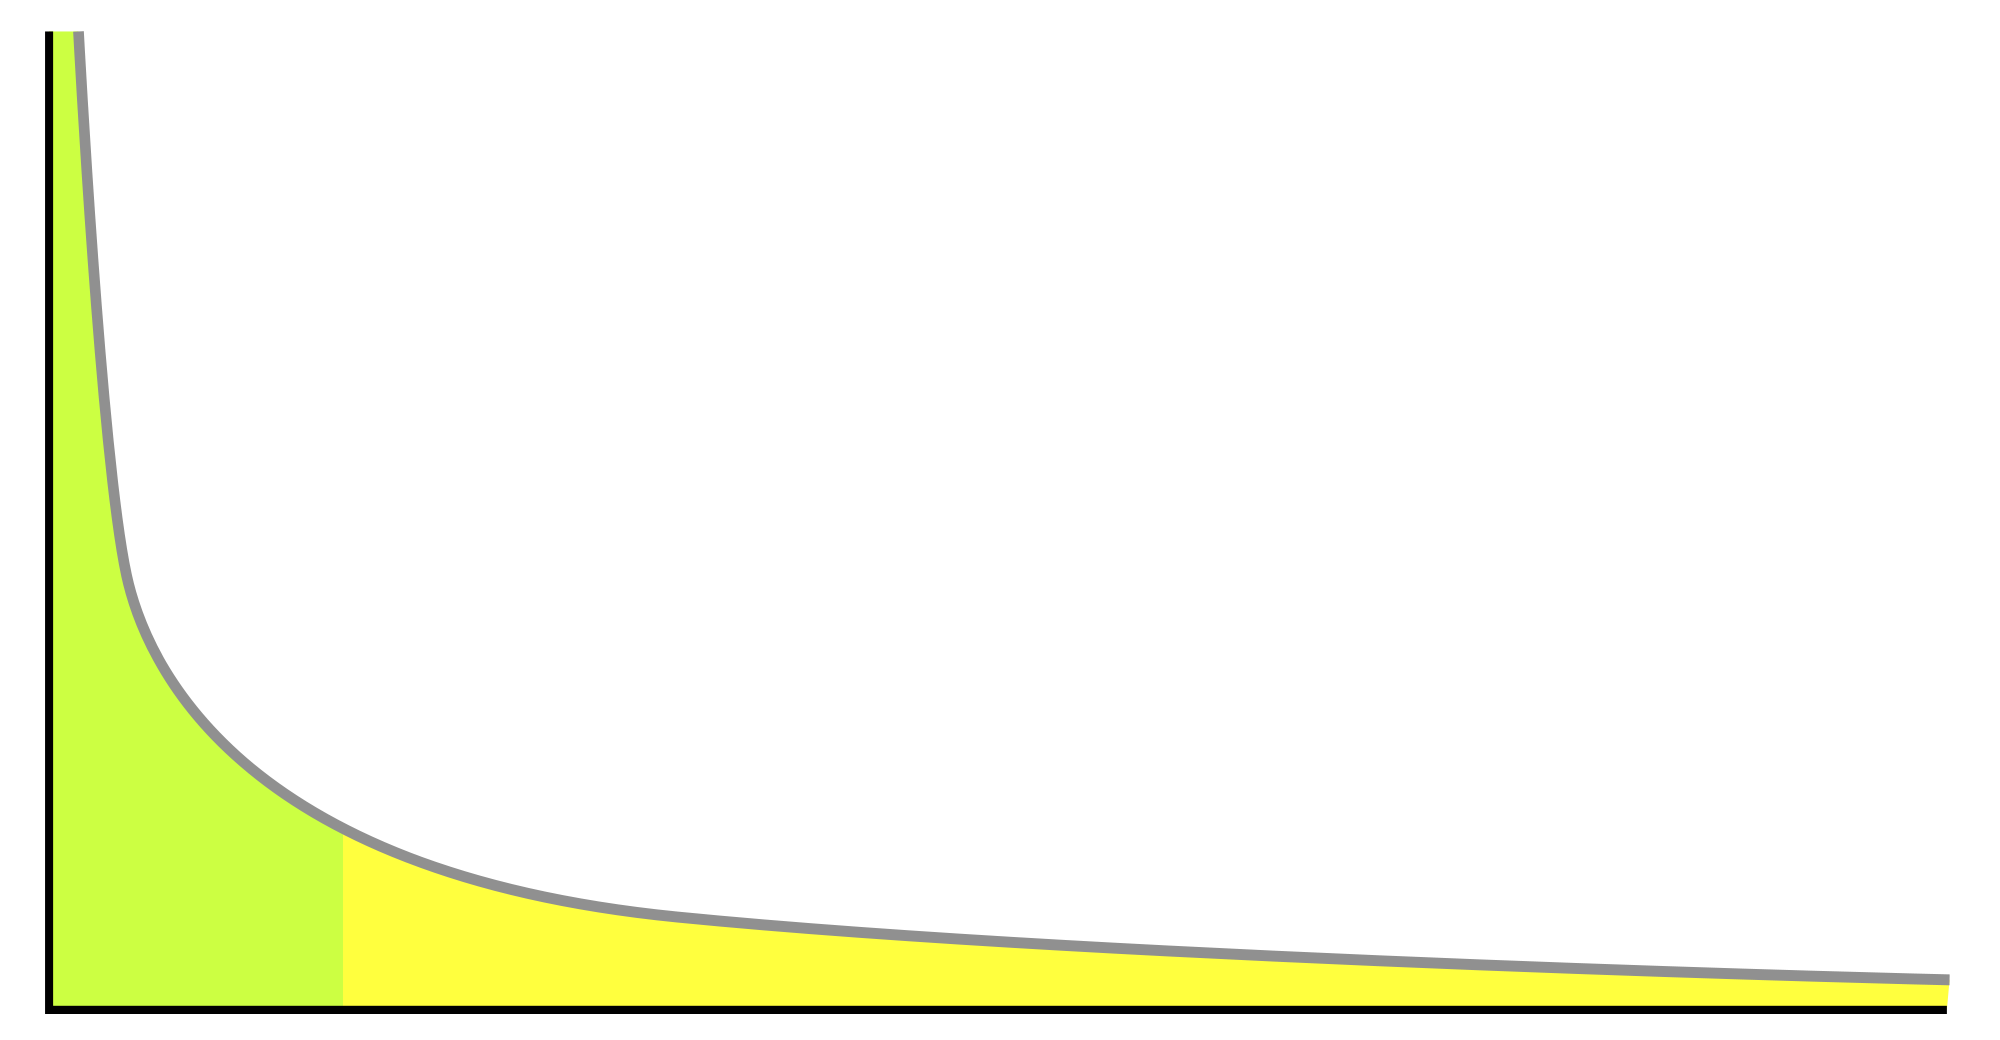
\includegraphics[width=0.8\textwidth]{obr/longtail.png}
 	\caption{Příklad rozdělení zobrazující popularitu hodnocení. Zdroj: \url{http://en.wikipedia.org/} \cite{wiki:longtail}}\label{fig:longtail}
\end{figure}	

	Všechny výše zmíněné faktory zapříčinily rozvoj přístupu zvaného \emph{informační filtrování}. Odtud už je jen krok k doporučování na míru, které se v posledních několika letech rozmohlo zaváděním tzv. \emph{doporučovacích systémů}.

	\subsection{Doporučovací systémy}
 Doporučovací systémy pracují s předem známými daty a mohou uživateli pomoci v tom smyslu, že z obrovské množiny informací různými způsoby vyfiltrují relevantní podmnožinu. Například sledováním a vyhodnocováním historie používání služby uživatelem (doposud nakoupené produkty, seznam všech jím ohodnocených článků či žebříček preferovaných hudebních interpretů) nebo porovnáváním kontextu uživatele s ostatními lidmi využívajících tu samou službu. Oběma způsoby je možné objevit pro uživatele zajímavé a jeho vkusu vyhovující položky.
	
	\subsubsection{Použití}
Kamkoliv se v dnešní době na internetu podíváme, máme velkou šanci, že na takovéto systémy narazíme. Mohou mít sice různá jména, například \emph{like}, \emph{lidé, které můžete znát} nebo třeba \emph{uživatelé kupující produkt X kupují též produkt Y}, ale všechny mají stejný význam, a to zaujmout či upozornit na něco či někoho konkrétního.Spousta elektronických obchodů, renomovaných aukčních domů, ale též serverů se zábavou na nich doslova staví svá podnikání. 
Sami jejich zákazníci navíc o doporučování stojí. Jsou vděční za navigaci a existuje vysoká pravděpodobnost, že dle ní budou provádět i své nákupy. Uživatelé ale nejsou hloupí – když dostávají špatná doporučení, odmítají je a ve výsledku odmítají celý systém.

Jako příklady úspěšně nasazených systémů lze uvést například doporučování zboží na serveru Amazon.com\footnote{Dle TODO je 35 procent prodaného zboží z předchozího doporučení.}, nabídka filmů na serveru Netflix\footnote{Dle TODO jsou 2/3 půjčených filmů z doporučení.} či různých článků z databází na internetu (CNN, Google News). 
	
	\subsubsection{Typy}
Doporučovací systémy lze dle způsobu práce rozdělit do dvou skupin. 

TODO

	behavioral (založeny na interakci uživatelů se články) - most popular, collabo. filter., item to item a content (založeny na článcích) - content similarity, latest item
	zmínit nejznámější doporučovací algoritmy, collaborative filtering, most popular, text similarity atd.
	ze treba pro potreby doporucovani novinek je lepsi kolaborativni filtrovani a ze pro doporucovani obsahu je lepsi text similarity

	\section{Motivace} 	
		
	Představme si nyní jakéhosi rádce, který dokáže v každém okamžiku rozhodnout, co je za daných okolností nejvhodnější. Rádce v klidu vyčkává, ale v okamžiku, kdy je tázán uživatelem na to, jakou metodou si má nechat doporučit obsah, aby z toho měl maximální užitek, je schopen ihned a bez dlouhého rozmýšlení odpovědět. Rádce dokáže i pružně reagovat na situaci, kdy náhle dojde ke změně preferencí či vyvstanou jiné nečekané události, které mají za následek doporučování nevhodného obsahu.
	
	\section{Projekt}
	Cílem práce tedy je navrhnout adaptibilní systém, který bude automaticky vhodně volit a kombinovat algoritmy. Bude využívat zpětnou vazbu ohledně kvality doporučení, která principem odměny za dobré doporučení nebo trestu za špatné ovlivní preference při kombinování. Zároveň bude zodpovědná za podporu velkého množství dotazujících se uživatelů.	
	
	Tato diplomová práce dokumentuje návrh a vývoj takového systému a s ním spolupracujících komponent.	
	
	Toto je seznam modulů, které byly pro potřeby práce vyvinuty:

\begin{itemize}
  \item \textbf{Adaptibilní systém pro doporučování obsahu.} The first item
  \item \textbf{Sada základních algoritmů určených k doporučování.} The second item
  \item \textbf{Rozhraní pro algoritmy a systému pro kombinování.} The third etc \ldots
\end{itemize}	

	\section{Struktura práce}
	Tato práce je strukturována do X různých kapitol a popisuje celý vývojový cyklus systému. Kapitoly jsou řazeny v tom samém pořadí, v jakém probíhaly vývojové fáze.	

\begin{description}
  \item[Kapitola] \nameref{chap:tests} The first item
  \item[Kapitola] \ref{chap:tests} The second item
  \item[Kapitola] The third etc \ldots
\end{description}
	
\end{introduction}

	
\chapter{Aktuální stav}	
Seznamte se s aktuálním stavem a proveďte rešerši.

\section{Existující řešení}


\section{Sada algoritmů}
Identifikujte sadu základních algoritmů určených pro kombinování. Ty implementujte nebo použijte existující implementace.

\chapter{Analýza}
\label{chap:analysis}
	
	\subsection{Real time}
	live read + live write = real time recommendation
	\url{http://www.slideshare.net/d0nut/realtime-recommender-with-redis-hands-on}	
			
\chapter{Adaptibilní systém}
Navrhněte, implementujte a otestujte systém, který bude dynamicky kombinovat algoritmy a optimalizovat celkovou kvalitu algoritmů.
\label{chap:ensemble}

\section{Strojové učení}

Vzhledem k povaze řešeného problému je nutné zaměřit se na metody tzv. \emph{strojového učení}. 
Jedná se o vědeckou disciplínu (jednu z větví oboru umělé inteligence), která se zabývá tím, jak se má počítač přizpůsobit určité situaci, aniž by byl pro danou situaci explicitně naprogramován. Metody strojového učení, které hledají generalizaci libovolných dat nebo slouží pro adaptaci existujícího systému na změny okolí, se používají ve všech oblastech informačních věd od analýzy snímků, analýzy DNA a textu, až po simulace chování člověka. 

Typickým příkladem je vytvořit z dostupných dat model, který dokáže:

\begin{itemize}
  \item predikovat cenu akcií za 6 měsíců z aktuální výkonnosti společnosti a ekonomických dat
  \item rozpoznat spam od regulérního e-mailu
  \item u pacienta hospitalizovaného s infarktem predikovat riziko dalšího infarktu
  \item napomoci společnostem zabývajících se internetovou reklamou v rozhodování se, kterou reklamní strategii použít k maximalizaci zisků
  Používá to ale třeba Google analytics! při správě online experimentů
\url{https://support.google.com/analytics/answer/2844870?hl=cs&ref_topic=2844866}
\end{itemize}

Algoritmy strojového učení mohou být děleny do taxonomie (nadtříd a podtříd) založené na požadovaném výsledku algoritmu nebo typu vstupu, který je k dispozici během trénování stroje. Algoritmů je celá řada, bude tedy vhodné zmínit zde alespoň ty nejtypičtější. 

\begin{description}
  \item[Supervised learning]~\footnote{učení s učitelem} TODO
  \item[Unsupervised learning]~\footnote{učení bez učitele} TODO
  \item[Reinforcement learning]~\footnote{zpětnovazební učení nebo též učení posilováním} TODO
\end{description}

TODO zmínit, že pro naše potřeby je nejvhodnější reinforcement learning.

Algoritmus začne ve stavu nevědomí (ignorant state), kdy neví nic o daných okolnostech a začíná nabývat vědomosti tím, že testuje systém. Tím, jak vstřebává data a vyhodnocuje výsledky, učí se, jaké chování je nejlepší.

Z psychologického hlediska se jedná o následující úvahu: Jakým způsobem dokáže trest a odměna ovlivňovat naše budoucí chování? Na základě čeho se (nejen) lidstvo učí novým věcem?

\subsection{Online učení}

Navrhovaná strategie je též nazývána jako \emph{online učení}. Nutno zmínit, že slovem online zde není míněno něco ve smyslu internetu, ale ve smyslu neustále se vyvíjející aktualizace dat. Učící algoritmus v každém kole vykoná nějakou akci, přijme zpětnou vazbu a připíše si daný zisk či ztrátu.

Z matematického hlediska má online učení propojení na klasické online algoritmy, teorii (opakovaných) her a teorii pravděpodobnosti. Díky těmto znalostem tak můžeme navrhovat pravděpodobností dynamické systémy, kterými lze modelovat složitá průmyslová zařízení nebo třeba výherní automat známý jako mnohoruký bandita (Multi-Armed Bandit).

\section{Multi-armed Bandit algoritmus}
The Multi-Armed Bandit Problem je jedním z klasických problémů online učení. Tato herní strategie je podobná tradičnímu hernímu automatu, který představuje one-armed strategii, ale mnohoruká varianta má více herních pák~\emph{V každém kole si lze pro hru vybírat mezi N automaty}. 

\subsection{Princip algoritmu}
Strategii si lze představit tak, že stojíme před N výherními automaty (též nazývány jako bandité) a v každém kole máme možnost vybrat si jeden z nich, na kterém budeme hrát. Pravděpodobnosti výher u jednotlivých automatů jsou pro nás neznámé. 

Formálně lze strategii popsat jako skupinu výnosových (reward) distribučních funkcí B = {R1, …, RK}, kde K je počet banditů. Každý bandita má tedy přiřazenu jednu distribuční funkci, jež vyjadřuje pravděpodobnost úspěchu. 

Zpočátku nemá hráč žádnou informaci o průběhu hry ani o rozložení pravděpodobnosti úspěchu napříč bandity. Tím, že v každém kole vybíráme vždy jen jednoho banditu, se snažíme navrhnout strategii pro maximalizaci celkové výhry.

Samozřejmě, že kdybychom znali banditu s největší pravděpodobností výhry, potom bychom jej vždy vybírali, čímž bychom maximalizovali výhry. Naším úkolem bude tedy nalézt nejlepšího banditu a to co nejrychleji, jak je to jen možné.

K návrhu strategie nám pomáhá to, že jednotlivé bandity nejdříve testujeme, abychom získali nutné znalosti. Poté už se lze zaměřovat na páky, které nám poskytují největší zužitkované znalosti. 

Úkol trochu komplikuje stochastická povaha banditů. Suboptimální bandita může vracet spoustu výher, což by nás mohlo přimět uvěřit, že právě tento bandita je velice štědrý. Podobně ale naopak nejlepší bandita může vracet spoustu proher. Měli bychom tedy pořád zkoušet i lůzry, nebo se na ně vykašlat?

Co je dalším problémem, tak pokud najdeme banditu, který vrací “docela dobré” výsledky, měli bychom toto zachovat a nadále rozvíjet naše “docela dobré” skóre, nebo bychom měli zkoušet i další bandity v naději, že nalezneme ještě lepšího? Tomuto se říká exploration vs. exploitation dilema.

NEMOJE
Nechť u1, …, uK jsou průměrné hodnoty výnosových distribučních funkcí. Hráč aktivně zatáhne za páku každé kolo a sleduje příslušný výnos. jeho úkolem je maximalizovat součet těchto výnosů. Oželení (regret) po T kolech je definováno jako rozdíl mezi součtem výnosů příslušných výnosových funkcí optimální strategie a součtu získaných výnosů (VZOREC VIZ kybernář)

\subsection{Exploration vs. Exploitation}

NEMOJE
Explorace 
Nacházení nových oblastí hledání - náhodné procházky, nevyužívá předchozích znalostí
Exploatace
Využití stávajících znalostí, uvíznutí v lokálních extrémech, rigidita

\section{Bayesian Bandits}

Ukazuje se ale, že nalézt optimální řešení je neuvěřitelně obtížné. A může trvat léta, než je celkové řešení vyvinuto. Existuje totiž také spousta přibližně optimálních řešení, které jsou docela dobré. 

Právě to jedno z mnoha takových řešení (které lze velice dobře škálovat) je známo jako Bayesian Bandits a bude se jednat o online algoritmus, o kterém už padla řeč v sekci \ref{} a má přímou souvislost s zpětnovazebním učením (reinforcement learning).

NEMOJE PRUBEH ALGORITMU
Bayesovské řešení začíná stanovením pravděpodobností výhry pro každého banditu z předchozích zkušeností. V našem případě jsou tyto pravděpodbnosti od 0 do 1. 

Prior a posterior by Verča
"před provedením pokusu" - např. pravděpodobnost, že hodím sudý číslo na kostce je 1/2, a "aposteriori" je po provedení pokusu - nedřív uděláš pokus - to se používa třeba u Bayesova vzorce. ale tý tabulce upřímně moc nerozumím... to prior má bejt asi jakože to, co předpokládáš, že bys měl mít a to posterior je, jak to jakože "odhadneš" třeba  zdat - jakože pokusem

V každém kole:
Vzorkování náhodné veličiny Xb 
Výběr bandity s největším vzorkem (např. vyber banditu B = argmax Xb)
Pozorujme výsledek vybrání bandity B a updatujme priors (takový ty prostě věci z dřívějšího vyhodnocování - pokusy a výhry)
Návrat na 1)

A to je vše. Z výpočetního hlediska algoritmus zahrnuje vzorkování z N distribucí. Počáteční priors jsou Beta(alfa = 1, beta = 1) (uniformní rozdělení) a pozorovaná náhodná veličina X (výhra či prohra, zakódována jako 1, respektive 0) je Binomialní, proto posterior (po provedení pokusu) je Beta(alfa = 1 + X, beta = 1 + 1 - X)

Takže pokud bychom měli odpovědět na otázku z dřívějška (zda vybírat i ty lůzry), tak tento algoritmus navrhuje to, abychom nevyřazovali lůzry, ale měli bychom je vybírat s klesajícím tempem, jakmile nashromáždíme dost jistoty, že existují lepší bandité. Vyplývá to z podstaty, že vždy existuje nenulová šance, že lůzr dosáhne statusu B, ale pravděpodobnost této události se snižuje s tím, jak hrajeme více kol. 

TODO možná nějaký obrázky (grafy) jak se to pulls vyvíjí (všechno je v článku na campdb)

Všimněme si, že se zase až tolik nestaráme o nějaké závěry nad skrytými pravděpodonostmi, spíše se pro tento problém zabýváme o výběr nejlepšího bandity (nebo přesnějšími slovy, stále jistějšího během vybírání banditů)

To je třeba vidět v tom grafu níže, že distribuce červeného bandity je velice široká (což představuje neznalost o tom, jaká by skrytá pravděpodobnost vůbec mohla být), ale jsme si docela dobře jistí, že není nejlepší, algoritmus se tedy rozhodne tohoto banditu ignorovat.

ZPETNA VAZBA
Multi-armed bandit je příklad Single-stage typu Reinforcement learningu (viz \url{https://cw.felk.cvut.cz/wiki/_media/courses/a3m33ui/prednasky/files/ui-2010-p11-reinforcement_learning.pdf}). Tedy snažíme se po jedné akci ihned uplatňovat feedback. Každá akce v multi-armed je nazývána jako jedna hra. Po každé hře at obdržíme (stochastický) reward t:
E[rt|at] = Q*(at) a z dlouhodobého hlediska je právě cílem maximalizovat reward.
“To solve the multi-armed bandit problem, one must explore a variety of
actions and exploit the best of them”

Q*(a) je “action-value odhad - v čitateli součet rewardu z jednotlivých výběrů / počet výběrů

Pak je ještě “greedy akce” ve hře t - at* = argmax Qt(a) 

Zajímavé poznámky
V případě jakéhokoliv úspěchu doporučení by se měla navýšit někde hodnota pravděpodobnosti, se kterou bude algoritmus znovu vybrán. V případě neúspěchu pak by se tato pravděpodobnost měla exponenciálně snížit. V další iteraci už se bude systém rozhodovat s touto pravděpodobnsotí mezí objevováním a zužitkováním. V případě zužitkování se vybírá z algoritmů, co již předtím něco vynesly. To je ta strategie learnable - u banditů to funguje tak, že poměr mezi objevováním a zužitkováním se mění v čase a ne v závislosti na předchozích výsledcích. Algoritmy jsou rozděleni ve svých dimenzích a každé té dimenzi je přiřazena určitá pravděpodbnost definující míru úspěšnosti nalezení toho, že tenhle algoritmus je fakt nejlepší. V případě, že uživatelé zužitkovávají tyto znalosti, tak si poté vybírají algoritmus, který má maximální pravděpodobnost z dané množiny. 
epsylog greedy!!!!! - varianta  epsylon decreasing
Jak to má kybernář: Je li pirát ve stavu objevování, tak v případě útoku na loď nalezne přísslušný prostor, který obsahuje místo útoku, a zvýší mu hodntou pravděpodbnosti. Když je ve stavu zužitkování znalostí, tak pluje do prostoru, kde hledá transportní lodě. V případě, že za celý cyklus nenalezne žádnou loď, tak se exponenciálně sníží hodnota pravděpodobnosti daného prostoru. Nalezne li loď,tak zvýšení pravděpodobnosti proběhne jako ve stavu objevování. 


ZAVEREM
Algoritmus je velice jednoduchý, proto je také jednoduché jej rozšířit. V mém případě bylo potřeba přidat learning rates - předpokládejme, že to prostředí se prostě může měnit v čase. Technicky by se tedy standardní Bayesian Bandit algoritmus self-updatoval tím, že by se učil tím, že to, co si myslel, že se zdá jako nejlepší, selhává nejčastěji. Také lze docílit toho, aby se algoritmus učil měnícím se prostředím rychleji. Potřebuje pro to jedinou věc - přidat rate napříč updatováním.

Pokud rate menší než 1, algoritmus bude zapomínat předchozí výsledky rychleji a tlak na neznalost bude směrem dolů. naopak rate větší než 1 implikuje to, že náě algoritmus se bude chovat více riskantně a bude vsázet na dřívější výhry častěji a bude tedy více odolný proti změnám měnícího se prostředí.
		
\chapter{Principy a technologie}
\label{chap:sysanalys}
Analýza a návrh systému pro kombinování metod pro doporučování obsahu v reálném čase
	\section{Vyhodnocovací technologie}	
	Výpočty. kvůli kombinování budeme počítat s floaty
	\section{Server}		
	Je třeba nějaký server, na kterém to bude běžet
	\section{Api}		
	
	\section{Jak to udělat, aby to běželo rychle?}		
	musíme zpracovávat data velice rychle
	rychlý webový server, rychlý síťový protokol, rychlou frontu zpráv, rychlé úložiště

\section{Principy a technologie technologií}
Sekce se zabývá výběrem vhodných technologií
REST, APlikační server, NoSQL, ZeroMQ, Hadoop, Apache mahout

\url{http://contest.plista.com/wiki/example}
\section{Architektura řešení}
\section{Návrh komunikace}
router, dealer, worker thready
\section{Parametrizace}
volba parametrů, ať už těch, co ovlivňují tresty nebo třeba úložiště (redis...)

\chapter{Návrh a implementace}
\label{chap:impl}
Realizace toho systému, jak jsem ty části propojil dohromady a tak

\section{Aplikace}
\section{Formát zasílaných zpráv}
\section{Komunikační protokol}
\section{Nasazení}
samotné aplikace, potom ještě rest api

\chapter{Experimenty a vyhodnocení}
\label{chap:tests}
kecy o testování
\section{Testování různých způsobů chování}
viz jak jarda vymyslel těch zhruba 5 příkladů, co mohou nastat
\section{Experimenty}

\section{Zhodnocení aplikace}
Slovní zhodnocení
\section{Budoucí práce}
bude li nějaká

\begin{conclusion}
	%sem napište závěr Vaší práce
\end{conclusion}

\bibliographystyle{csn690}
\bibliography{mybibliographyfile}

\appendix

\chapter{Seznam použitých zkratek}
% \printglossaries
\begin{description}
	\item[GUI] Graphical user interface
	\item[XML] Extensible markup language
\end{description}


% % % % % % % % % % % % % % % % % % % % % % % % % % % % 
% % Tuto kapitolu z výsledné práce ODSTRAŇTE.
% % % % % % % % % % % % % % % % % % % % % % % % % % % % 
% 
% \chapter{Návod k~použití této šablony}
% 
% Tento dokument slouží jako základ pro napsání závěrečné práce na Fakultě informačních technologií ČVUT v~Praze.
% 
% \section{Výběr základu}
% 
% Vyberte si šablonu podle druhu práce (bakalářská, diplomová), jazyka (čeština, angličtina) a kódování (ASCII, \mbox{UTF-8}, \mbox{ISO-8859-2} neboli latin2 a nebo \mbox{Windows-1250}). 
% 
% V~české variantě naleznete šablony v~souborech pojmenovaných ve formátu práce\_kódování.tex. Typ může být:
% \begin{description}
% 	\item[BP] bakalářská práce,
% 	\item[DP] diplomová (magisterská) práce.
% \end{description}
% Kódování, ve kterém chcete psát, může být:
% \begin{description}
% 	\item[UTF-8] kódování Unicode,
% 	\item[ISO-8859-2] latin2,
% 	\item[Windows-1250] znaková sada 1250 Windows.
% \end{description}
% V~případě nejistoty ohledně kódování doporučujeme následující postup:
% \begin{enumerate}
% 	\item Otevřete šablony pro kódování UTF-8 v~editoru prostého textu, který chcete pro psaní práce použít -- pokud můžete texty s~diakritikou normálně přečíst, použijte tuto šablonu.
% 	\item V~opačném případě postupujte dále podle toho, jaký operační systém používáte:
% 	\begin{itemize}
% 		\item v~případě Windows použijte šablonu pro kódování \mbox{Windows-1250},
% 		\item jinak zkuste použít šablonu pro kódování \mbox{ISO-8859-2}.
% 	\end{itemize}
% \end{enumerate}
% 
% 
% V~anglické variantě jsou šablony pojmenované podle typu práce, možnosti jsou:
% \begin{description}
% 	\item[bachelors] bakalářská práce,
% 	\item[masters] diplomová (magisterská) práce.
% \end{description}
% 
% \section{Použití šablony}
% 
% Šablona je určena pro zpracování systémem \LaTeXe{}. Text je možné psát v~textovém editoru jako prostý text, lze však také využít specializovaný editor pro \LaTeX{}, např. Kile.
% 
% Pro získání tisknutelného výstupu z~takto vytvořeného souboru použijte příkaz \verb|pdflatex|, kterému předáte cestu k~souboru jako parametr. Vhodný editor pro \LaTeX{} toto udělá za Vás. \verb|pdfcslatex| ani \verb|cslatex| \emph{nebudou} s~těmito šablonami fungovat.
% 
% Více informací o~použití systému \LaTeX{} najdete např. v~\cite{wikilatex}.
% 
% \subsection{Typografie}
% 
% Při psaní dodržujte typografické konvence zvoleného jazyka. České \uv{uvozovky} zapisujte použitím příkazu \verb|\uv|, kterému v~parametru předáte text, jenž má být v~uvozovkách. Anglické otevírací uvozovky se v~\LaTeX{}u zadávají jako dva zpětné apostrofy, uzavírací uvozovky jako dva apostrofy. Často chybně uváděný symbol "{} (palce) nemá s~uvozovkami nic společného.
% 
% Dále je třeba zabránit zalomení řádky mezi některými slovy, v~češtině např. za jednopísmennými předložkami a spojkami (vyjma \uv{a}). To docílíte vložením pružné nezalomitelné mezery -- znakem \texttt{\textasciitilde}. V~tomto případě to není třeba dělat ručně, lze použít program \verb|vlna|.
% 
% Více o~typografii viz \cite{kobltypo}.
% 
% \subsection{Obrázky}
% 
% Pro umožnění vkládání obrázků je vhodné použít balíček \verb|graphicx|, samotné vložení se provede příkazem \verb|\includegraphics|. Takto je možné vkládat obrázky ve formátu PDF, PNG a JPEG jestliže používáte pdf\LaTeX{} nebo ve formátu EPS jestliže používáte \LaTeX{}. Doporučujeme preferovat vektorové obrázky před rastrovými (vyjma fotografií).
% 
% \subsubsection{Získání vhodného formátu}
% 
% Pro získání vektorových formátů PDF nebo EPS z~jiných lze použít některý z~vektorových grafických editorů. Pro převod rastrového obrázku na vektorový lze použít rasterizaci, kterou mnohé editory zvládají (např. Inkscape). Pro konverze lze použít též nástroje pro dávkové zpracování běžně dodávané s~\LaTeX{}em, např. \verb|epstopdf|.
% 
% \subsubsection{Plovoucí prostředí}
% 
% Příkazem \verb|\includegraphics| lze obrázky vkládat přímo, doporučujeme však použít plovoucí prostředí, konkrétně \verb|figure|. Například obrázek \ref{fig:float} byl vložen tímto způsobem. Vůbec přitom nevadí, když je obrázek umístěn jinde, než bylo původně zamýšleno -- je tomu tak hlavně kvůli dodržení typografických konvencí. Namísto vynucování konkrétní pozice obrázku doporučujeme používat odkazování z~textu (dvojice příkazů \verb|\label| a \verb|\ref|).
% 
% \begin{figure}\centering
% 	
\includegraphics[width=0.5\textwidth, angle=30]{cvut-logo-bw}
% 	\caption[Příklad obrázku]{Ukázkový obrázek v~plovoucím prostředí}\label{fig:float}
% \end{figure}
% 
% \subsubsection{Verze obrázků}
% 
% % Gnuplot BW i barevně
% Může se hodit mít více verzí stejného obrázku, např. pro barevný či černobílý tisk a nebo pro prezentaci. S~pomocí některých nástrojů na generování grafiky je to snadné.
% 
% Máte-li například graf vytvořený v programu Gnuplot, můžete jeho černobílou variantu (viz obr. \ref{fig:gnuplot-bw}) vytvořit parametrem \verb|monochrome dashed| příkazu \verb|set term|. Barevnou variantu (viz obr. \ref{fig:gnuplot-col}) vhodnou na prezentace lze vytvořit parametrem \verb|colour solid|.
% 
% \begin{figure}\centering
% 	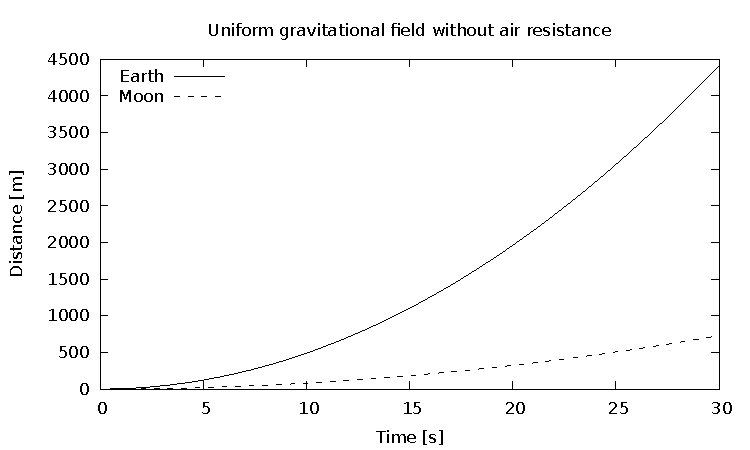
\includegraphics{gnuplot-bw}
% 	\caption{Černobílá varianta obrázku generovaného programem Gnuplot}\label{fig:gnuplot-bw}
% \end{figure}
% 
% \begin{figure}\centering
% 	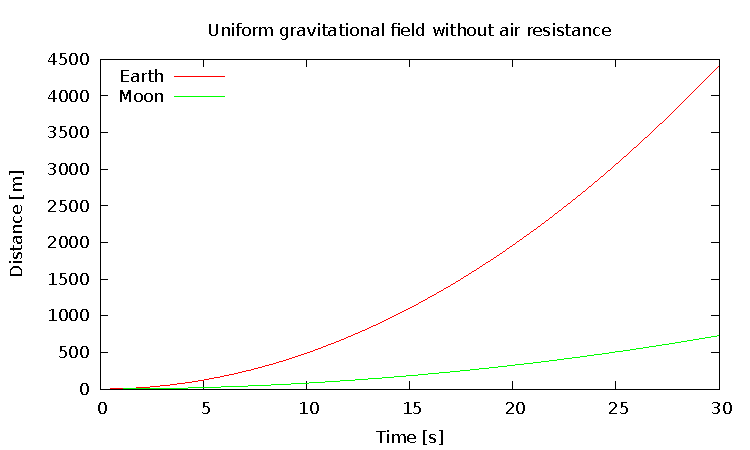
\includegraphics{gnuplot-col}
% 	\caption{Barevná varianta obrázku generovaného programem Gnuplot}\label{fig:gnuplot-col}
% \end{figure}
% 
% 
% \subsection{Tabulky}
% 
% Tabulky lze zadávat různě, např. v~prostředí \verb|tabular|, avšak pro jejich vkládání platí to samé, co pro obrázky -- použijte plovoucí prostředí, v~tomto případě \verb|table|. Například tabulka \ref{tab:matematika} byla vložena tímto způsobem.
% 
% \begin{table}\centering
% 	\caption[Příklad tabulky]{Zadávání matematiky}\label{tab:matematika}
% 	\begin{tabular}{|l|l|c|c|}\hline
% 		Typ		& Prostředí		& \LaTeX{}ovská zkratka	& \TeX{}ovská zkratka	\tabularnewline \hline \hline
% 		Text		& \verb|math|		& \verb|\(...\)|	& \verb|$...$|		\tabularnewline \hline
% 		Displayed	& \verb|displaymath|	& \verb|\[...\]|	& \verb|$$...$$|	\tabularnewline \hline
% 	\end{tabular}
% \end{table}
% 
% % % % % % % % % % % % % % % % % % % % % % % % % % % % 

\chapter{Obsah přiloženého CD}

%upravte podle skutecnosti

\begin{figure}
	\dirtree{%
		.1 readme.txt\DTcomment{stručný popis obsahu CD}.
		.1 exe\DTcomment{adresář se spustitelnou formou implementace}.
		.1 src.
		.2 impl\DTcomment{zdrojové kódy implementace}.
		.2 thesis\DTcomment{zdrojová forma práce ve formátu \LaTeX{}}.
		.1 text\DTcomment{text práce}.
		.2 thesis.pdf\DTcomment{text práce ve formátu PDF}.
		.2 thesis.ps\DTcomment{text práce ve formátu PS}.
	}
\end{figure}

\end{document}
